\section{Magnesium Borohydride [$\beta-$\ce{Mg(BH4)2}]}
\label{sec:borohydrides-magnesium}

The calculational supercell was relaxed, from the $fddd$ spacegroup ($\#70$), totalling 176 atoms.
The structure consists of 5 symmetry inequivelant \ce{BH4} sites which all have similar local structure, being wedged between 2 \ce{Mg} atoms (\fref{fig:mg-local-structure}).
The symmetry inequivilance stems from the fact that each \ce{BH4} was slightly away from the \ce{Mg}-\ce{Mg} axis.
The distance, $L$, from the \ce{B} to the axis, influences the barriers.

\begin{figure}
\begin{center}
%\figmiss{Environment, for explaining the axes used}
    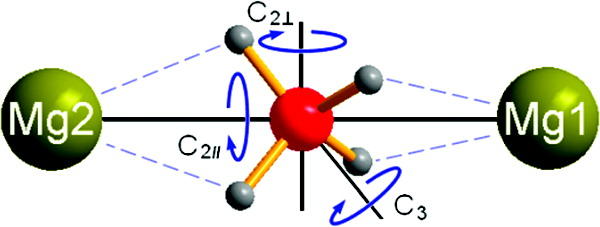
\includegraphics[width=1.0\linewidth]{mg-local-structure}
\caption{Schematic representation of the environment of each \ce{B} atom, and how the different types of axes relates to it.
\tred{Temporary graphics}
}
\label{fig:mg-local-structure}
\end{center}
\end{figure}

The experimental data detected only rotational diffusion.
Thus, the work exclusively revolved around understanding which rotations correpsonded with the experiments.

For each inequivelant site a number of rigid rotation PESes were constructed\footnote{Examples of which can be seen in figures 13 and 14 of paper \ref{pap:magnesium}} in order to get an overview of the interesting events and to limit computations spent on the MEP calculations, similar to \fref{sec:borohydrides-calcium}.
Due to symmetry not all the axes needed to be considered.

The general result from the PESes was that rotations that maximised the \ce{Mg}-\ce{H}, $d_{H-Mg}$ distance showed the lowest energies (\fref{fig:h-mg-distances}).
In this respect, two distinct types of $C_2$ axes were seen, those parallel to the \ce{Mg}-\ce{Mg} axis, $C_2^\parallel$, which maximised $d_{H-Mg}$ and those perpendicular to it, $C_2^\perp$, where $d_{H-Mg}$ was generally lower and had higher barriers.
MEP calculations for the latter found a combination of other axes yielded the same permutation but at a much lower energy cost.
The difference in relative barrier height decreased with decreasing $L$.\footnote{The relative difference would be non-existant for $L=0$ but non of the \ce{BH4} fulfill that critrion.}

\begin{figure}[h]
\begin{center}
  \subfigure[Average \ce{H}-\ce{Mg} distance]{
    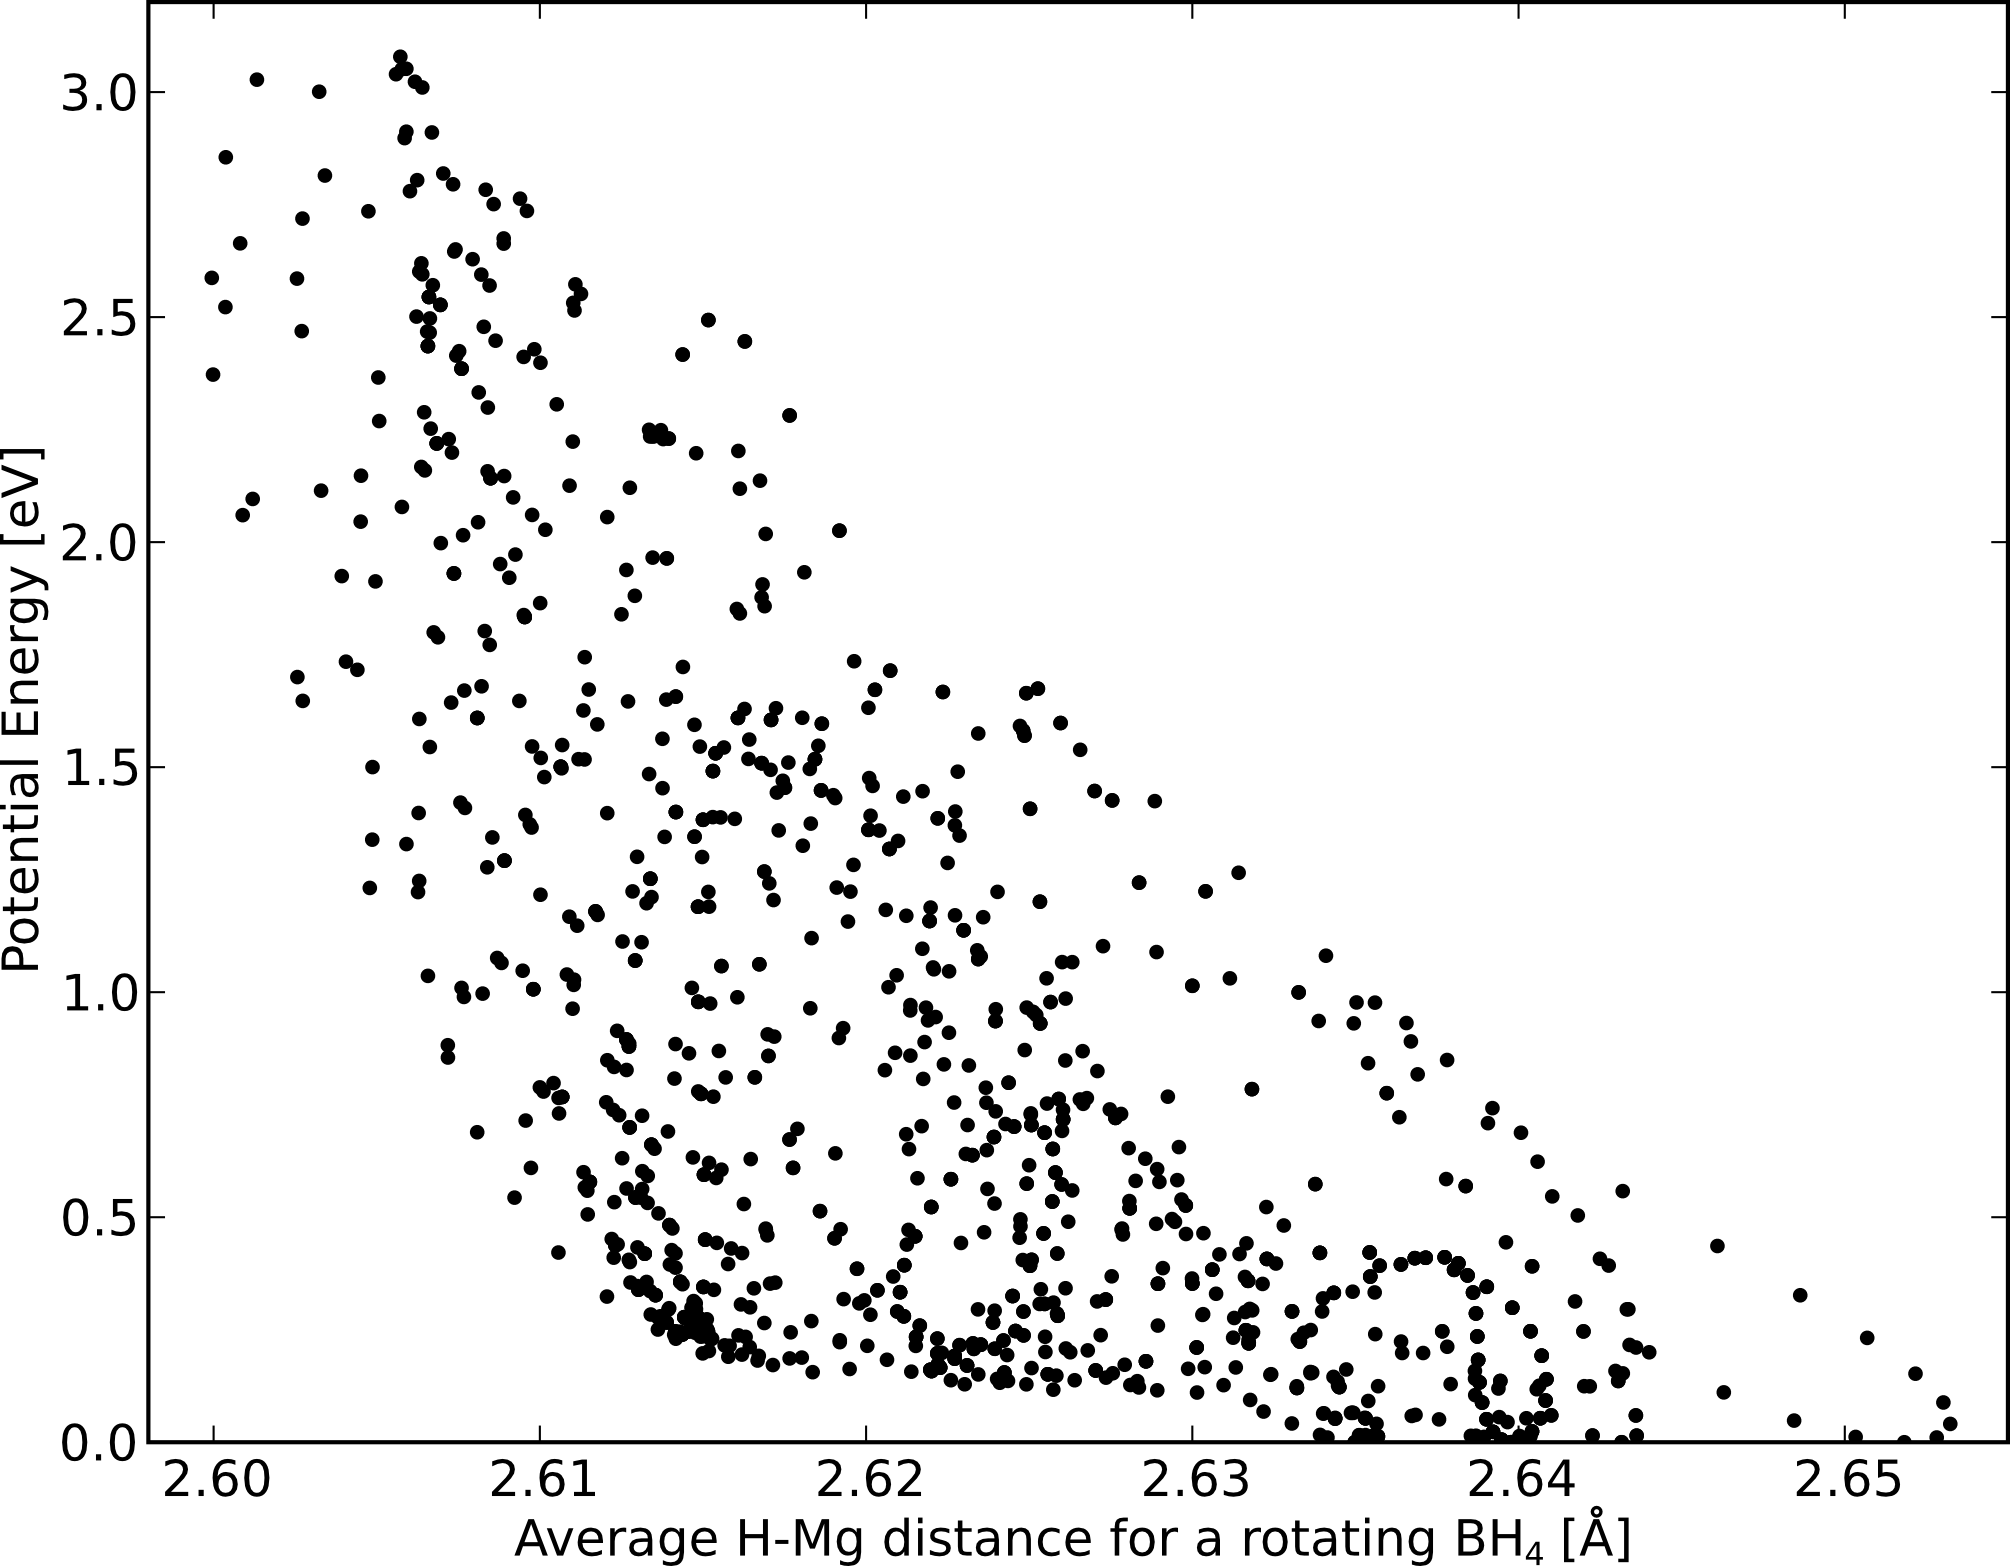
\includegraphics[width=0.45\linewidth]{h-mg-distances-avg}
    \label{fig:h-mg-distances-avg}
    }
  \subfigure[Minimum \ce{H}-\ce{Mg} distance]{
    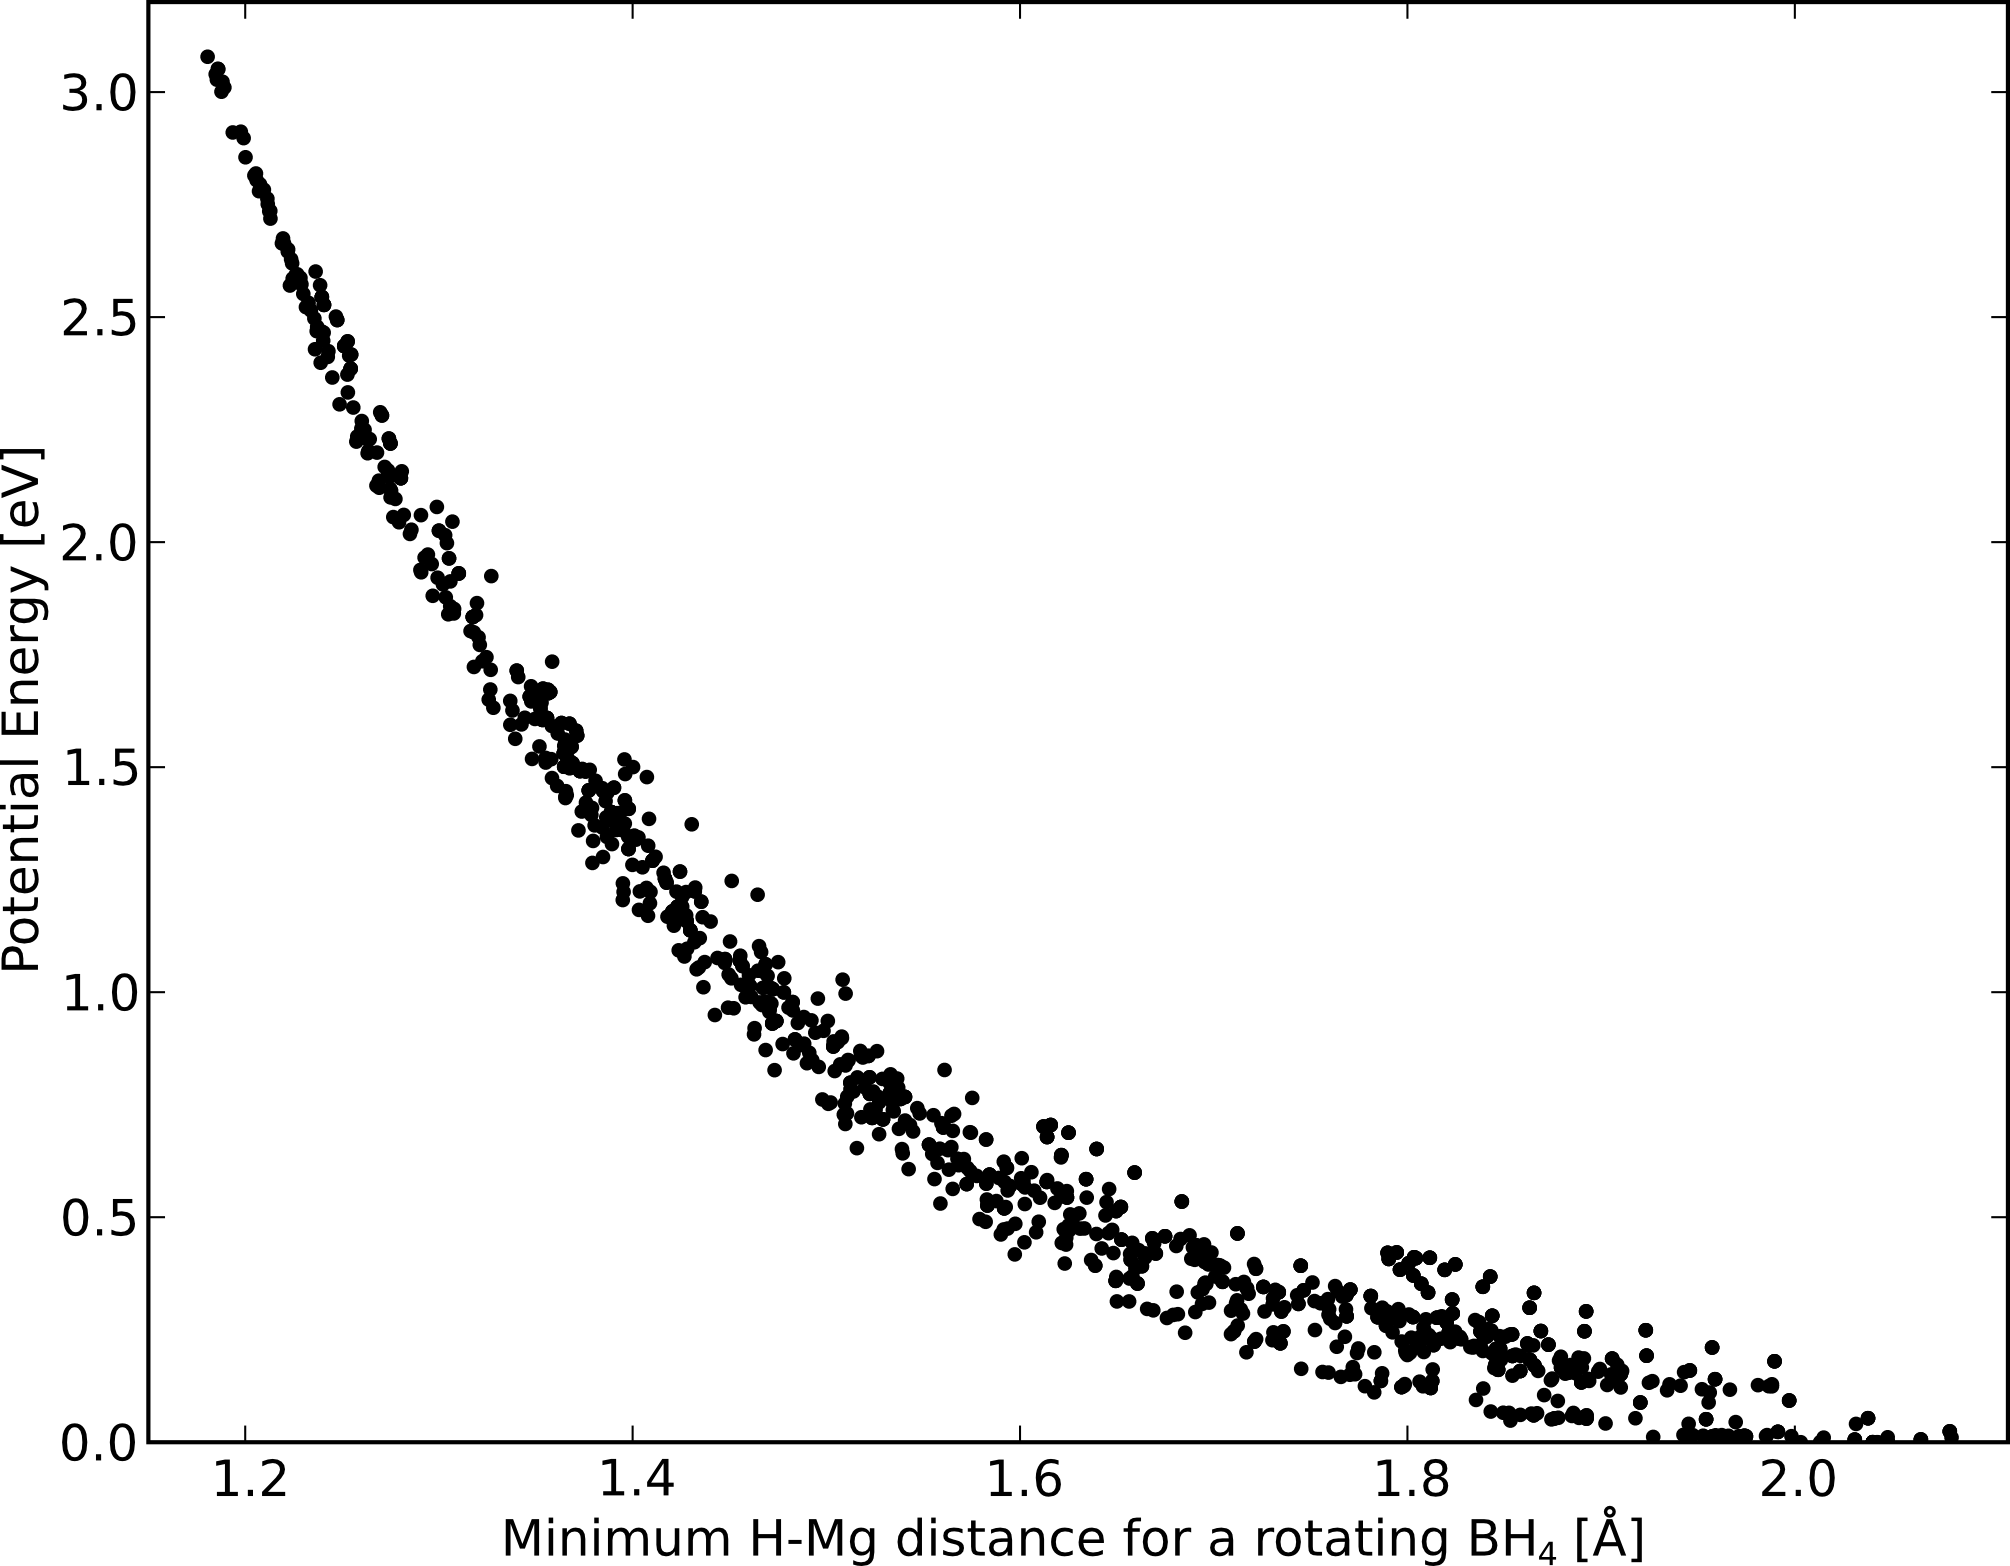
\includegraphics[width=0.45\linewidth]{h-mg-distances-min}
    \label{fig:h-mg-distances-min}
    }
    \parbox{0.85\linewidth}{
      \caption{For each PES, the distances between the \ce{H} atoms of the rotating \ce{BH4} unit to the neighboring \ce{Mg} atoms is plotted.
Some systematic features can be seen since the data was produced with specific rotations rather than a uniform distirubtion.
A clear trend for lower energies with higher distances can be seen.
      }
      \label{fig:h-mg-distances}
    }
\end{center}
\end{figure}

No such clear distinction could be made with regards to the $C_3$ axes.
However, due to symmetry all the $C_3$ axes for a given site yield a very similar PES.

The rigid rotation plots are not able to give a full description of the events, neither their geometry nor their energetics.
Thus MEP calculations were performed with the lowest energy rigid rotation paths as starting positions.

\begin{figure}
\begin{center}
  \subfigure[The rotational energy barriers for \ce{BH4} in $\beta$-\ce{Mg(BH4)2}][The energy barriers as a function of $L$, the distance from the \ce{B} to the \ce{Mg}-\ce{Mg} axis.
The circles are the $C_2$ barriers, while the triangles are the $C_3$ axes.
A clear linear relationship (the line) can be seen for the $C_2$ axes.
]{
    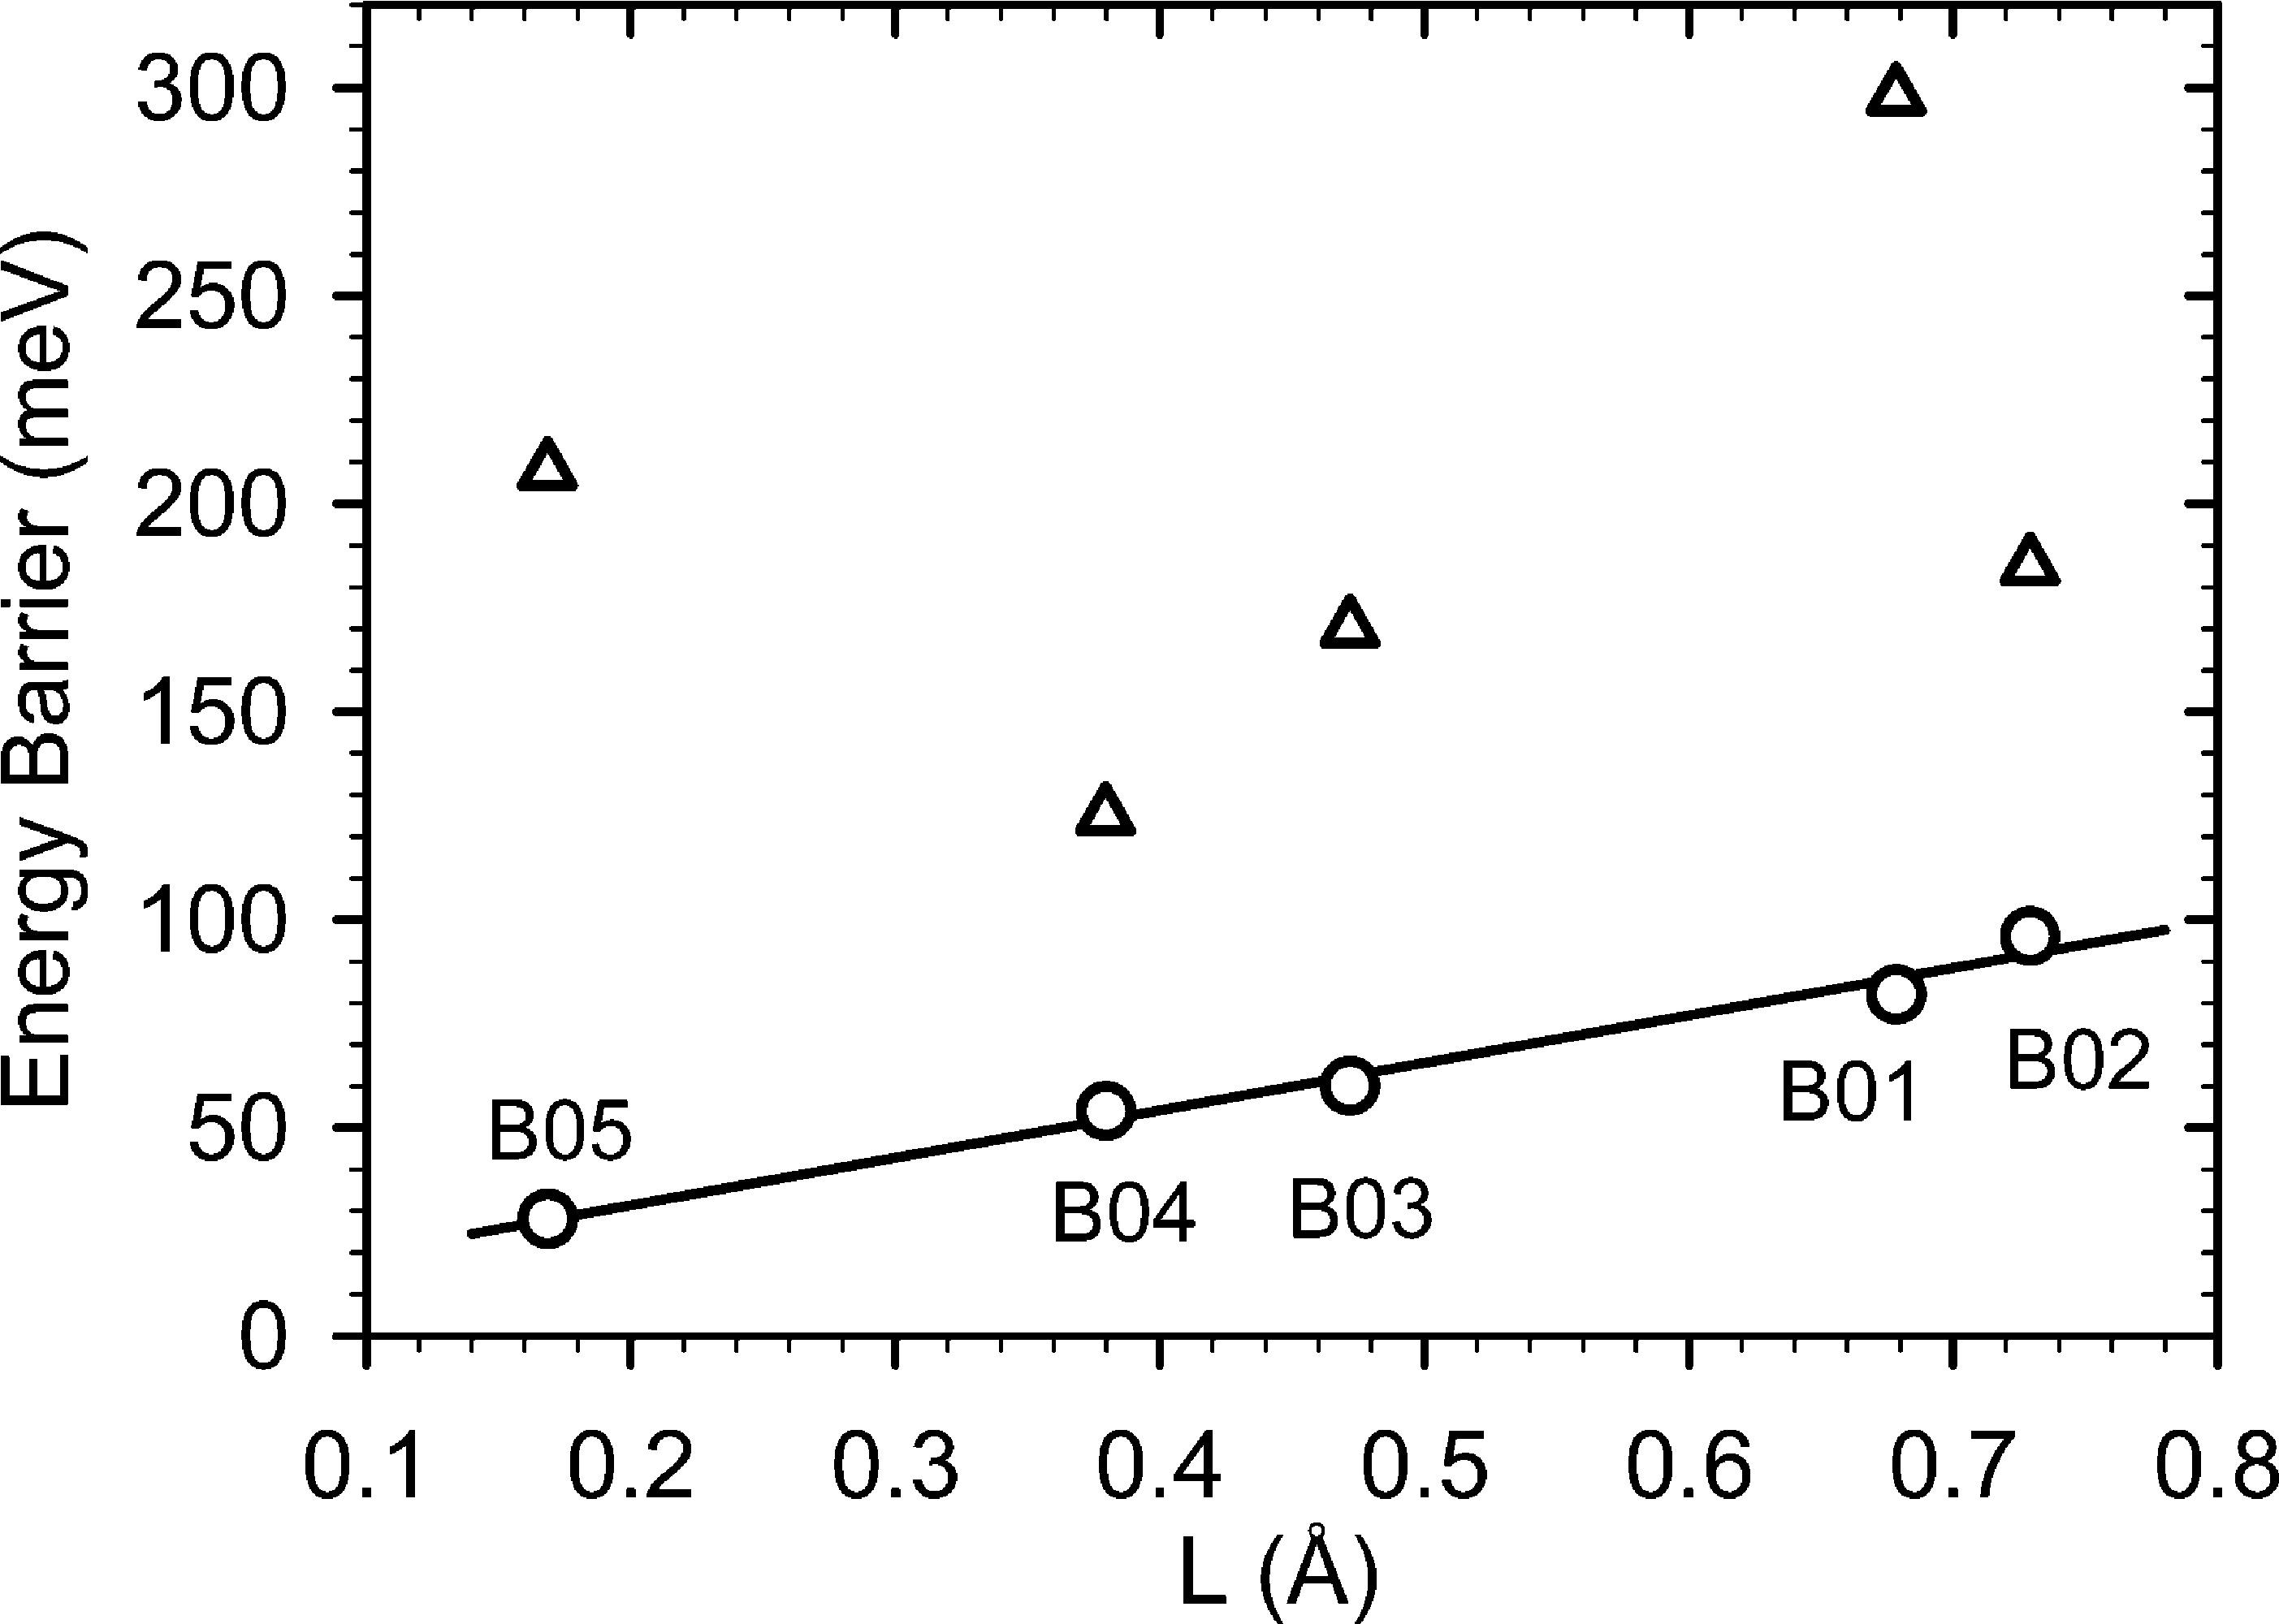
\includegraphics[width=0.45\linewidth]{mg-barriers}
%\figmiss{Barrier dependancy on distance}
    \label{fig:mg-barriers}
    }
  \subfigure[Comparison of the experimental and theoretical results][\expand]{
    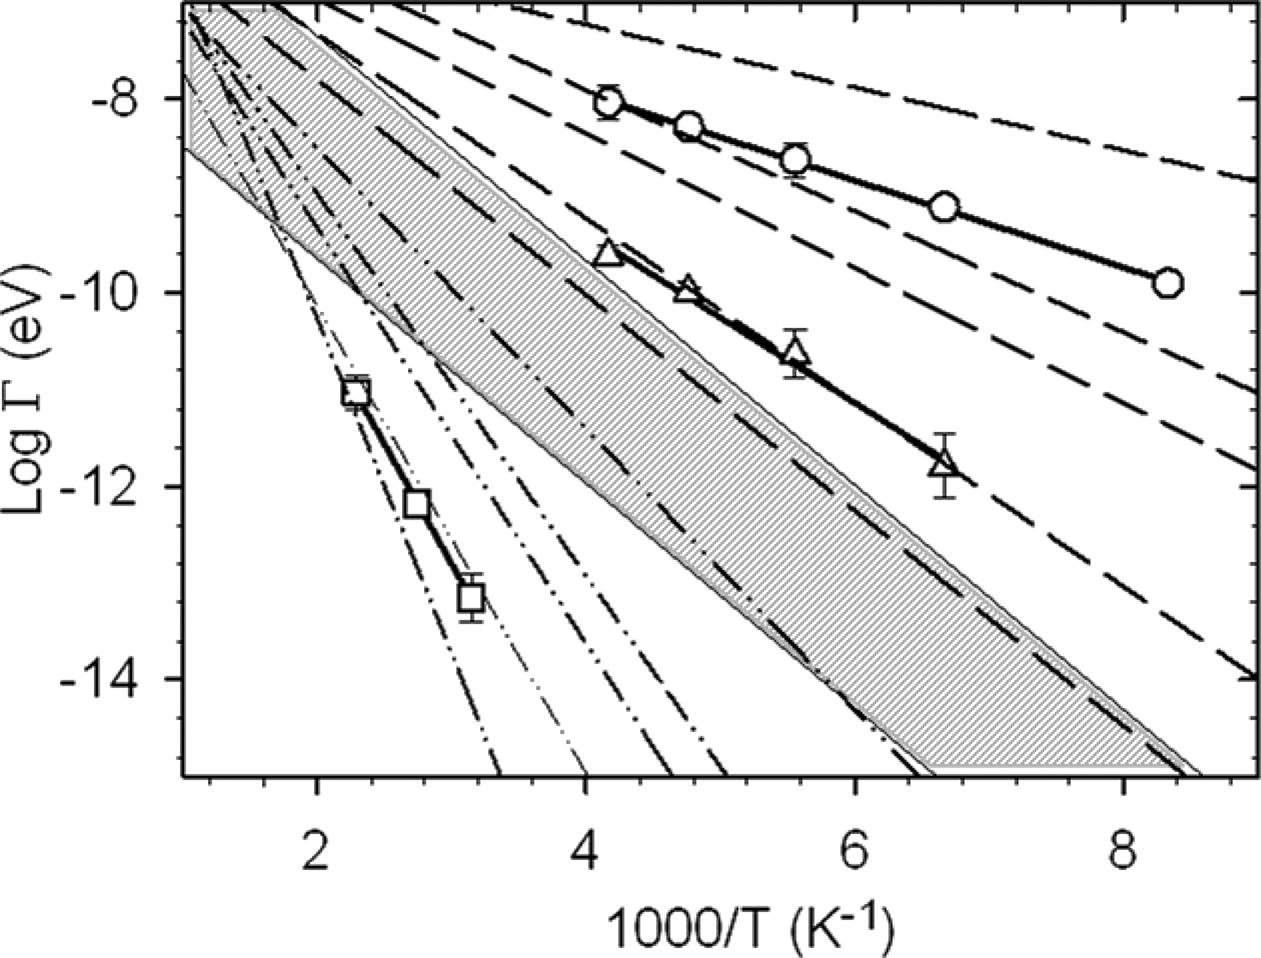
\includegraphics[width=0.45\linewidth]{mg-experimental-comparison}
%\figmiss{Comparison of the experimental and theoretical results}
    \label{fig:mg-experimental-comaprison}
    }
\caption{The main results for $\beta$-\ce{Mg(BH4)2} 
\tred{Temporary graphics}
}
\label{fig:mg-results}
\end{center}
\end{figure}

It is unsurprising to find that there is, in fact, a direct relationship between $L$ and the $C_2$ barrier height.
In fact, the relationship is linear, as can be seen in \fref{fig:mg-barriers}, the barrier increases with increased $L$ which is most likely due more \ce{H}-\ce{Mg} interaction.
On the other hand, no such direct relationship could be found for the $C_3$ axes.



